\documentclass[
  12pt,
  openright,
  twoside,
  a4paper,
  english,
  brazil
]{abntex2}

\usepackage{indentfirst}
\usepackage{pdfpages}
\usepackage[alf]{abntex2cite}

\titulo{Implementação de um front end para IR LLVM}
\tituloestrangeiro{Implementing a LLVM IR front end}

\autor{Bernardo Ferrari Mendonça}
\local{Brasil}
\data{2019}
\orientador{Rafael de Santiago}
\coorientador{Evandro}
\instituicao{
  Universidade Federal de Santa Catarina
  \par
  Departamento de Informática e Estatística
  \par
  Ciência da Computação
}

\tipotrabalho{Trabalho de Conclusão de Curso de Graduação}

\preambulo{Proposta de monografia submetida ao Programa
de Graduação em Ciência da Computação
para a obtenção do Grau de Bacharel.}

\begin{document}
\pretextual{}
\imprimircapa{}
\imprimirfolhaderosto{}

\begin{folhadeaprovacao}
  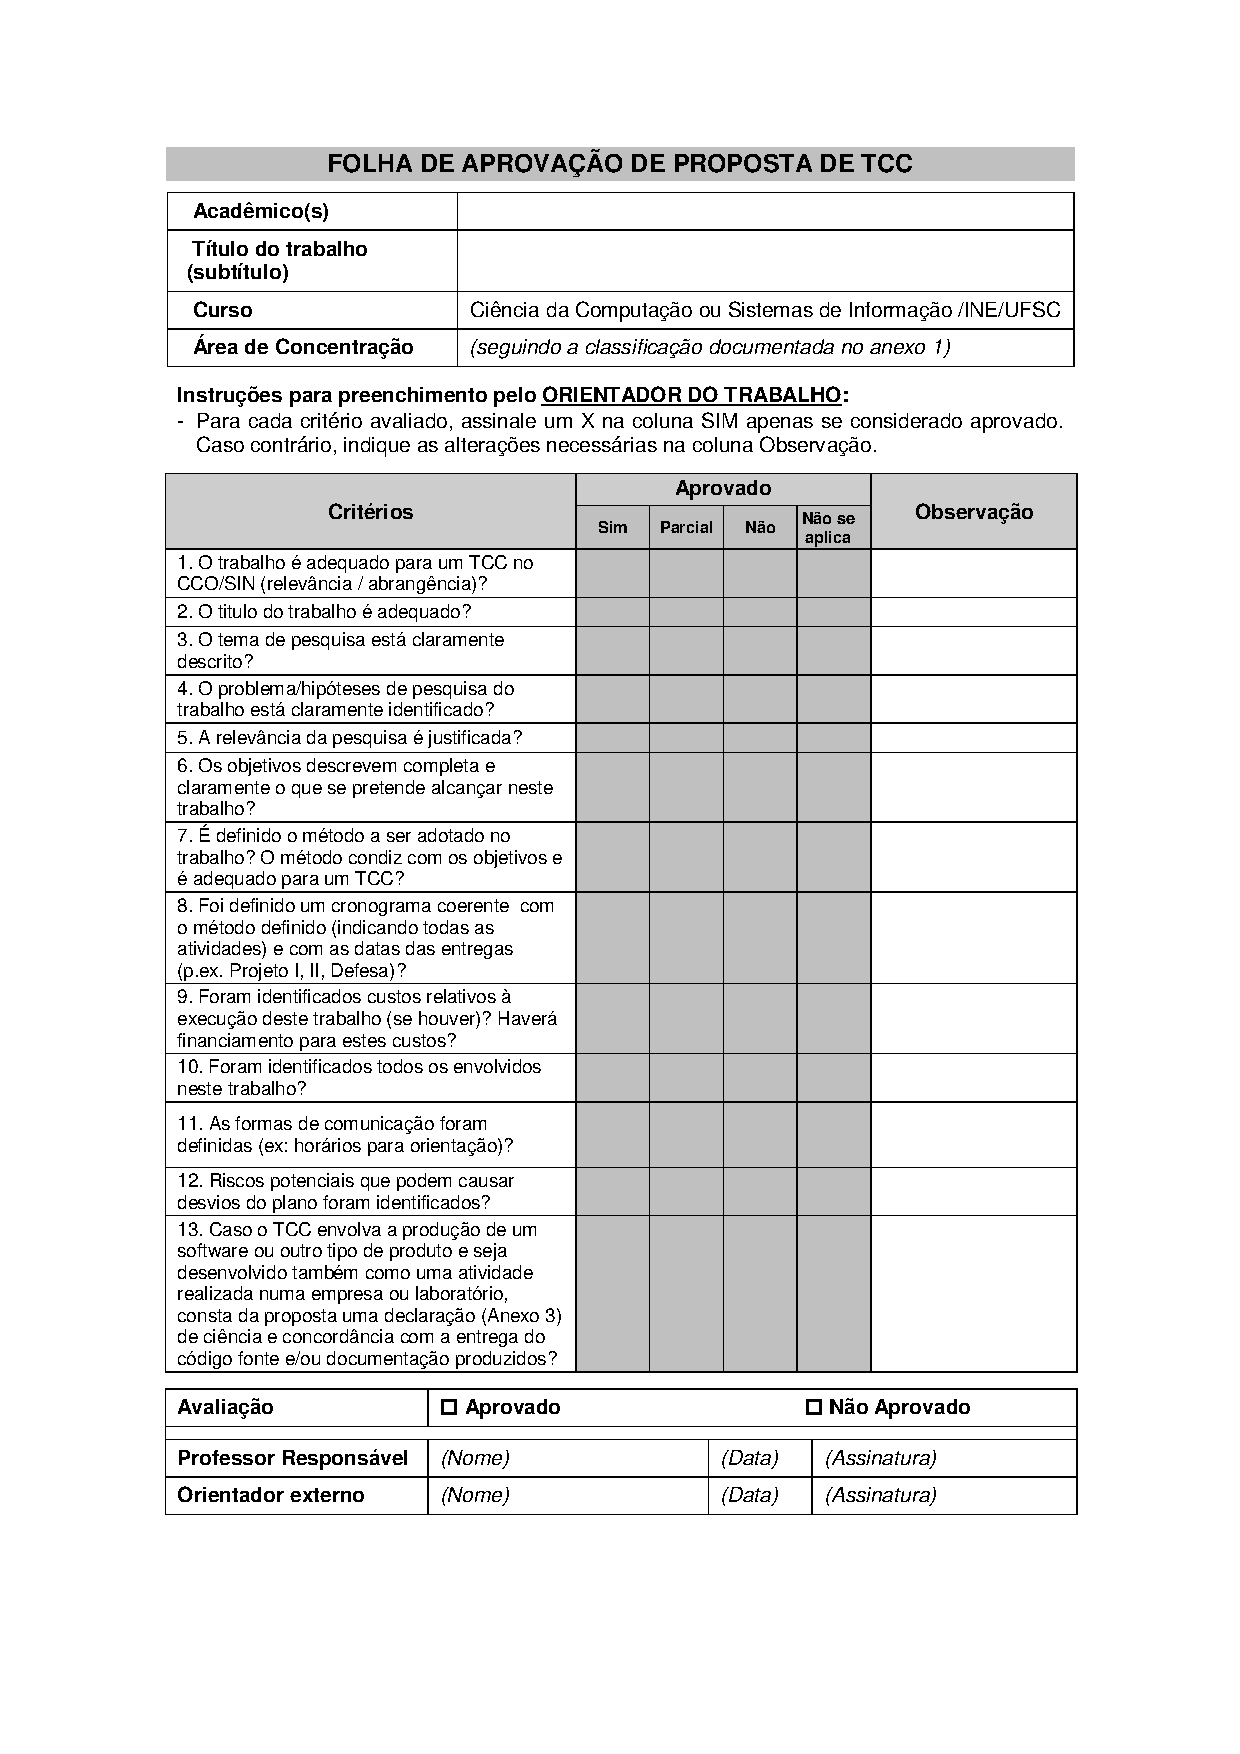
\includepdf{folha-de-aprovacao.pdf}
\end{folhadeaprovacao}

\begin{resumo}
Meu resumo.

\vspace{\onelineskip}
\noindent
\textbf{Palavras-chave}: minhas\@. palavras\@. chave.

\end{resumo}

\begin{KeepFromToc}
  \tableofcontents
\end{KeepFromToc}

\textual{}

\chapter{Introdução}\label{cap:introdução}

Esta vai ser minha introdução\cite{dijkstra1968}!
Este é outro paragrafo!

\postextual{}

\bibliography{bibliography.bib}

\end{document}
